\documentclass{standalone}
\usepackage{tikz}
\usetikzlibrary{shapes.misc, arrows.meta, positioning, bending, fit}

\begin{document}
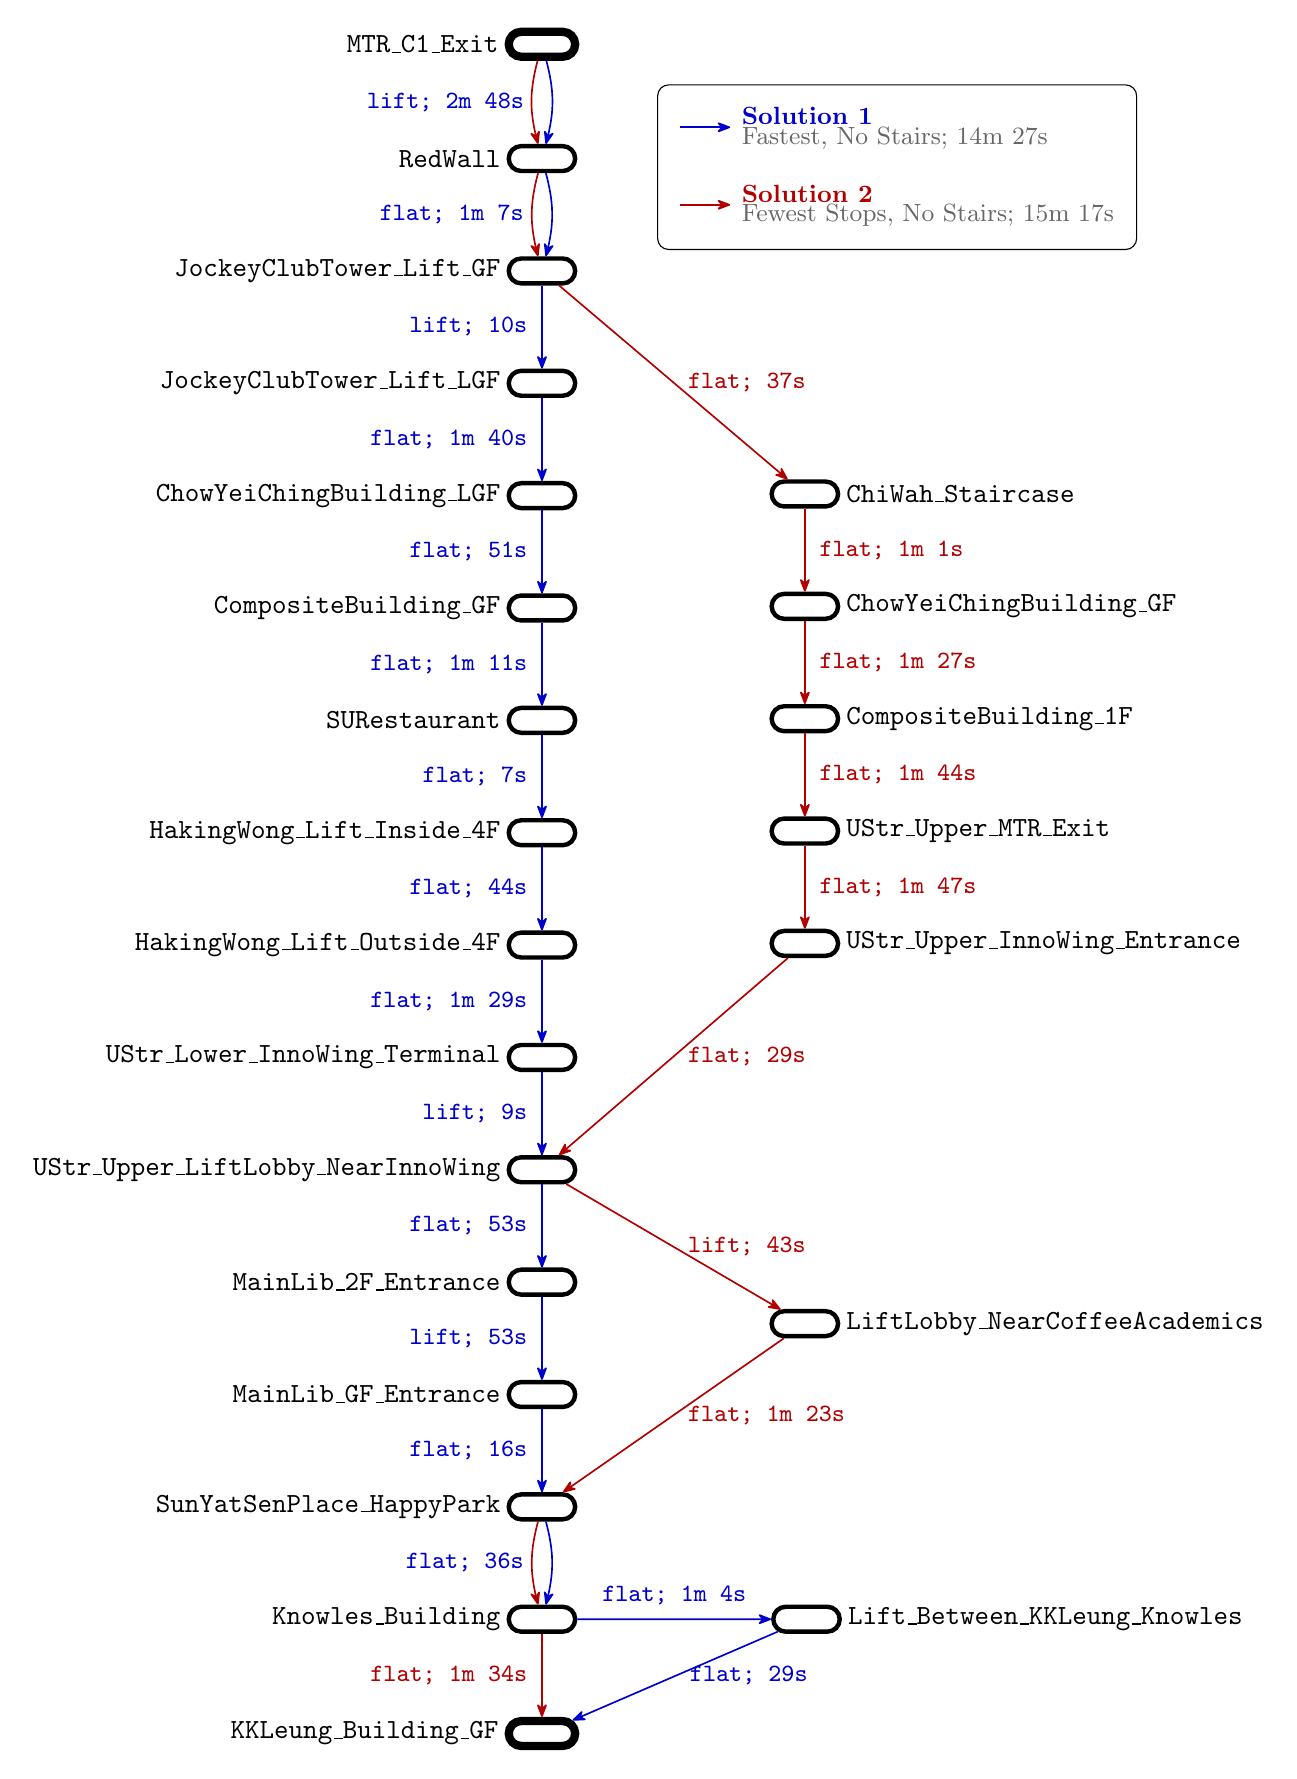
\begin{tikzpicture}[
    %% ── Node styles ──────────────────────────────────────────────────────
    %%
    %% station: small pill/stadium shape used as the "dot" indicator.
    %%   The node body is EMPTY; the monospaced name lives OUTSIDE as a label.
    %%   Edges and positioning are anchored to the pill shape, not the text.
    %%
    %%   Usage:
    %%     \node[station, label={[stlabel]right:NODE\_ID}]               (A) {};
    %%     \node[station-bold, label={[stlabel-bold]right:NODE\_ID}]     (A) {};
    %%
    station/.style={
        draw,
        shape=rounded rectangle,   % from shapes.misc — true semi-circular ends
        rounded rectangle arc length=180,
        minimum height=0.9em,       % height sets the semicircle diameter
        minimum width=2.4em,        % must exceed height to get a flat middle section
        inner xsep=0pt,
        inner ysep=0pt,
        line width=1.6pt
    },
    %% station-bold + stlabel-bold: use on start/end/waypoint nodes for emphasis.
    station-bold/.style={station, line width=3pt},
    %% stlabel: monospaced name label placed to the right of the station dot.
    %%   Always pass it as the style argument to the label option:
    %%     label={[stlabel]right:NAME}
    stlabel/.style={font=\ttfamily, inner sep=2pt},
    stlabel-bold/.style={stlabel, font=\ttfamily\bfseries},
    %% ── Base directed edge style ───────────────────────────────────────────────
    %%
    %%   All per-solution styles inherit from this.
    %%   For parallel edges use bend left/right:
    %%     \draw[sol1, bend left=20] (A) to node[elabel, above] {label} (B);
    route/.style={
        ->,
        >=Stealth[round],
        semithick,
        % shorten >=4pt,
        % shorten <=4pt,
    },
    %% ── Per-solution edge styles (one colour per solution) ────────────
    %%
    %%   Usage:  \draw[sol1] (A) -- (B);
    %%           \draw[sol2, bend left=20] (A) to node[elabel, above] {text} (B);
    sol1/.style={route, color=blue!80!black},           % Solution 1 — blue
    sol2/.style={route, color=red!70!black},            % Solution 2 — red
    sol3/.style={route, color=green!55!black},          % Solution 3 — green
    sol4/.style={route, color=orange!85!black},         % Solution 4 — orange
    sol5/.style={route, color=violet!80!black},         % Solution 5 — violet
    %% ── Edge label styles ────────────────────────────────────────────────
    %%
    %%   Use the per-solution variant (elabel1–elabel5) so that identical labels
    %%   on parallel edges are still distinguishable by colour.
    %%
    %%   For N parallel edges on the same node pair, spread them symmetrically:
    %%     N=2: bend left=15  /  bend right=15
    %%     N=3: bend left=25  /  straight (no bend)  /  bend right=25
    %%     N=4: bend left=35  /  bend left=12  /  bend right=12  /  bend right=35
    %%
    %%   To additionally separate labels, use xshift on the node option:
    %%     node[elabel3, right, xshift=8pt]
    %%
    %%   Example (2 parallel edges):
    %%     \draw[sol1, bend left=15]  (A) to node[elabel1, left]  {label} (B);
    %%     \draw[sol2, bend right=15] (A) to node[elabel2, right] {label} (B);
    %% ── Legend styles ──────────────────────────────────────────────────────
    %%
    %%   legendtitle: bold coloured solution name — pair with the solution colour.
    %%     e.g. \node[legendtitle, text=blue!80!black] {Solution 1};
    legendtitle/.style={font=\small\bfseries, inner sep=0pt, anchor=west},
    %%   legenddesc: smaller grey text for the lines below the title.
    legenddesc/.style={font=\small, text=black!60, inner sep=0pt, anchor=west},
    elabel/.style ={font=\small\ttfamily, inner sep=5pt},
    elabel1/.style={elabel, text=blue!80!black},
    elabel2/.style={elabel, text=red!70!black},
    elabel3/.style={elabel, text=green!55!black},
    elabel4/.style={elabel, text=orange!85!black},
    elabel5/.style={elabel, text=violet!80!black},
]

%% ── Shared prefix nodes ──────────────────────────────────────────────────
%%   Both routes: MTR_C1_Exit → RedWall → JockeyClubTower_Lift_GF

\node[station-bold, label={[stlabel-bold]left:MTR\_C1\_Exit}]
    (MTR_C1_Exit) {};
\node[station, label={[stlabel]left:RedWall},
    below=30pt of MTR_C1_Exit]
    (RedWall) {};
\node[station, label={[stlabel]left:JockeyClubTower\_Lift\_GF},
    below=30pt of RedWall]
    (JockeyClubTower_Lift_GF) {};

%% Sol1 spine (left column) ───────────────────────────────────────────────
%%   JockeyClubTower_Lift_GF → JockeyClubTower_Lift_LGF → ... → MainLib_GF_Entrance

\node[station, label={[stlabel]left:JockeyClubTower\_Lift\_LGF},
    below=30pt of JockeyClubTower_Lift_GF]
    (JockeyClubTower_Lift_LGF) {};
\node[station, label={[stlabel]left:ChowYeiChingBuilding\_LGF},
    below=30pt of JockeyClubTower_Lift_LGF]
    (ChowYeiChingBuilding_LGF) {};
\node[station, label={[stlabel]left:CompositeBuilding\_GF},
    below=30pt of ChowYeiChingBuilding_LGF]
    (CompositeBuilding_GF) {};
\node[station, label={[stlabel]left:SURestaurant},
    below=30pt of CompositeBuilding_GF]
    (SURestaurant) {};
\node[station, label={[stlabel]left:HakingWong\_Lift\_Inside\_4F},
    below=30pt of SURestaurant]
    (HakingWong_Lift_Inside_4F) {};
\node[station, label={[stlabel]left:HakingWong\_Lift\_Outside\_4F},
    below=30pt of HakingWong_Lift_Inside_4F]
    (HakingWong_Lift_Outside_4F) {};
\node[station, label={[stlabel]left:UStr\_Lower\_InnoWing\_Terminal},
    below=30pt of HakingWong_Lift_Outside_4F]
    (UStr_Lower_InnoWing_Terminal) {};
\node[station, label={[stlabel]left:UStr\_Upper\_LiftLobby\_NearInnoWing},
    below=30pt of UStr_Lower_InnoWing_Terminal]
    (UStr_Upper_LiftLobby_NearInnoWing) {};  %% Sol2 also merges here
\node[station, label={[stlabel]left:MainLib\_2F\_Entrance},
    below=30pt of UStr_Upper_LiftLobby_NearInnoWing]
    (MainLib_2F_Entrance) {};
\node[station, label={[stlabel]left:MainLib\_GF\_Entrance},
    below=30pt of MainLib_2F_Entrance]
    (MainLib_GF_Entrance) {};

%% Shared tail nodes ──────────────────────────────────────────────────────

\node[station, label={[stlabel]left:SunYatSenPlace\_HappyPark},
    below=30pt of MainLib_GF_Entrance]
    (SunYatSenPlace_HappyPark) {};
\node[station, label={[stlabel]left:Knowles\_Building},
    below=30pt of SunYatSenPlace_HappyPark]
    (Knowles_Building) {};
\node[station-bold, label={[stlabel-bold]left:KKLeung\_Building\_GF},
    below=30pt of Knowles_Building]
    (KKLeung_Building_GF) {};

%% Sol1 via Lift_Between_KKLeung_Knowles (right of Knowles_Building) ──────

\node[station, label={[stlabel]right:Lift\_Between\_KKLeung\_Knowles},
    right=70pt of Knowles_Building]
    (Lift_Between_KKLeung_Knowles) {};

%% Sol2 detour (right column, branching from JockeyClubTower_Lift_GF) ─────
%%   JockeyClubTower_Lift_GF → ChiWah_Staircase → ... → UStr_Upper_InnoWing_Entrance
%%   → UStr_Upper_LiftLobby_NearInnoWing (merge with Sol1 spine)
%%   → LiftLobby_NearCoffeeAcademics → SunYatSenPlace_HappyPark

\node[station, label={[stlabel]right:ChiWah\_Staircase},
    below right=70pt and 80pt of JockeyClubTower_Lift_GF]
    (ChiWah_Staircase) {};
\node[station, label={[stlabel]right:ChowYeiChingBuilding\_GF},
    below=30pt of ChiWah_Staircase]
    (ChowYeiChingBuilding_GF) {};
\node[station, label={[stlabel]right:CompositeBuilding\_1F},
    below=30pt of ChowYeiChingBuilding_GF]
    (CompositeBuilding_1F) {};
\node[station, label={[stlabel]right:UStr\_Upper\_MTR\_Exit},
    below=30pt of CompositeBuilding_1F]
    (UStr_Upper_MTR_Exit) {};
\node[station, label={[stlabel]right:UStr\_Upper\_InnoWing\_Entrance},
    below=30pt of UStr_Upper_MTR_Exit]
    (UStr_Upper_InnoWing_Entrance) {};

%% Sol2: UStr_Upper_LiftLobby_NearInnoWing → LiftLobby_NearCoffeeAcademics
\node[station, label={[stlabel]right:LiftLobby\_NearCoffeeAcademics},
    below right=45pt and 80pt of UStr_Upper_LiftLobby_NearInnoWing]
    (LiftLobby_NearCoffeeAcademics) {};

%% ── Edges ────────────────────────────────────────────────────────────────

%% Shared prefix: both routes (N=2)
\draw[sol1, bend left=15]  (MTR_C1_Exit) to node[elabel1, left, xshift=-5pt]  {lift; 2m 48s} (RedWall);
\draw[sol2, bend right=15] (MTR_C1_Exit) to (RedWall);

\draw[sol1, bend left=15]  (RedWall) to node[elabel1, left, xshift=-5pt]  {flat; 1m 7s} (JockeyClubTower_Lift_GF);
\draw[sol2, bend right=15] (RedWall) to (JockeyClubTower_Lift_GF);

%% Sol1: JockeyClubTower_Lift_GF → JockeyClubTower_Lift_LGF (lift) → spine
\draw[sol1] (JockeyClubTower_Lift_GF)    -- node[elabel1, left]  {lift; 10s}     (JockeyClubTower_Lift_LGF);
\draw[sol1] (JockeyClubTower_Lift_LGF)   -- node[elabel1, left]  {flat; 1m 40s}  (ChowYeiChingBuilding_LGF);
\draw[sol1] (ChowYeiChingBuilding_LGF)   -- node[elabel1, left]  {flat; 51s}     (CompositeBuilding_GF);
\draw[sol1] (CompositeBuilding_GF)       -- node[elabel1, left]  {flat; 1m 11s}  (SURestaurant);
\draw[sol1] (SURestaurant)               -- node[elabel1, left]  {flat; 7s}      (HakingWong_Lift_Inside_4F);
\draw[sol1] (HakingWong_Lift_Inside_4F)  -- node[elabel1, left]  {flat; 44s}     (HakingWong_Lift_Outside_4F);
\draw[sol1] (HakingWong_Lift_Outside_4F) -- node[elabel1, left]  {flat; 1m 29s}  (UStr_Lower_InnoWing_Terminal);
\draw[sol1] (UStr_Lower_InnoWing_Terminal) -- node[elabel1, left] {lift; 9s}     (UStr_Upper_LiftLobby_NearInnoWing);
\draw[sol1] (UStr_Upper_LiftLobby_NearInnoWing) -- node[elabel1, left] {flat; 53s}  (MainLib_2F_Entrance);
\draw[sol1] (MainLib_2F_Entrance)        -- node[elabel1, left]  {lift; 53s}     (MainLib_GF_Entrance);
\draw[sol1] (MainLib_GF_Entrance)        -- node[elabel1, left]  {flat; 16s}     (SunYatSenPlace_HappyPark);

%% Sol2: JockeyClubTower_Lift_GF → detour right column → UStr_Upper_LiftLobby_NearInnoWing
\draw[sol2] (JockeyClubTower_Lift_GF)    -- node[elabel2, right] {flat; 37s}     (ChiWah_Staircase);
\draw[sol2] (ChiWah_Staircase)           -- node[elabel2, right] {flat; 1m 1s}   (ChowYeiChingBuilding_GF);
\draw[sol2] (ChowYeiChingBuilding_GF)    -- node[elabel2, right] {flat; 1m 27s}  (CompositeBuilding_1F);
\draw[sol2] (CompositeBuilding_1F)       -- node[elabel2, right] {flat; 1m 44s}  (UStr_Upper_MTR_Exit);
\draw[sol2] (UStr_Upper_MTR_Exit)        -- node[elabel2, right] {flat; 1m 47s}  (UStr_Upper_InnoWing_Entrance);
\draw[sol2] (UStr_Upper_InnoWing_Entrance) --
    node[elabel2, right] {flat; 29s} (UStr_Upper_LiftLobby_NearInnoWing);
\draw[sol2] (UStr_Upper_LiftLobby_NearInnoWing) -- node[elabel2, right] {lift; 43s}   (LiftLobby_NearCoffeeAcademics);
\draw[sol2] (LiftLobby_NearCoffeeAcademics)     -- node[elabel2, right] {flat; 1m 23s} (SunYatSenPlace_HappyPark);

%% Shared tail: SunYatSenPlace_HappyPark → Knowles_Building (N=2, same cost)
\draw[sol1, bend left=15]  (SunYatSenPlace_HappyPark) to node[elabel1, left, xshift=-5pt] {flat; 36s} (Knowles_Building);
\draw[sol2, bend right=15] (SunYatSenPlace_HappyPark) to (Knowles_Building);

%% Sol1: Knowles_Building → Lift_Between_KKLeung_Knowles → KKLeung_Building_GF
\draw[sol1] (Knowles_Building)            -- node[elabel1, above] {flat; 1m 4s}  (Lift_Between_KKLeung_Knowles);
\draw[sol1] (Lift_Between_KKLeung_Knowles) -- node[elabel1, right] {flat; 29s}  (KKLeung_Building_GF);

%% Sol2: Knowles_Building → KKLeung_Building_GF (direct)
\draw[sol2] (Knowles_Building) -- node[elabel2, left] {flat; 1m 34s} (KKLeung_Building_GF);

%% ── Legend ───────────────────────────────────────────────────────────────

\begin{scope}[shift={(50pt, -30pt)}]
    \node[inner sep=0, minimum size=0] (leg-orig) at (0, 0) {};
    \draw[sol1] (0, 0) -- (1.8em, 0);
    \node[legendtitle, text=blue!80!black]  (li1-title) at (2.2em,  0.4em) {Solution 1};
    \node[legenddesc]                       (li1-desc)  at (2.2em, -0.4em) {Fastest, No Stairs; 14m 27s};

    \draw[sol2] (0, -2.8em) -- (1.8em, -2.8em);
    \node[legendtitle, text=red!70!black]   (li2-title) at (2.2em, -2.8em+0.4em) {Solution 2};
    \node[legenddesc]                       (li2-desc)  at (2.2em, -2.8em-0.4em) {Fewest Stops, No Stairs; 15m 17s};

    \node[draw, rounded corners=4pt, inner sep=8pt,
          fit=(leg-orig)(li1-title)(li1-desc)(li2-title)(li2-desc)
    ] {};
\end{scope}

\end{tikzpicture}
\end{document}
